\documentclass[10pt,pdf,hyperref={unicode}]{beamer}

\usepackage[normalem]{ulem}
\usepackage{qrcode}
\usepackage{array}
\usepackage[T2A]{fontenc}
\usepackage[utf8]{inputenc}
\usepackage{colortbl}
\usepackage{minted}
\usepackage{listings}
\usepackage{tcolorbox}

\setbeamertemplate{navigation symbols}{}

\usetheme{default}

\usepackage{array}
\newcolumntype{L}[1]{>{\raggedright\let\newline\\\arraybackslash\hspace{0pt}}m{#1}}
\newcolumntype{C}[1]{>{\centering\let\newline\\\arraybackslash\hspace{0pt}}m{#1}}
\newcolumntype{R}[1]{>{\raggedleft\let\newline\\\arraybackslash\hspace{0pt}}m{#1}}

\definecolor{shadecolor}{RGB}{210,210,210}
\newcommand{\asm}[1]{\mintinline{gas}{#1}}

\newcommand{\qrlinkframe}[2]{\begin{frame}{#1}
\center\qrcode[hyperlink,height=75px]{#2}
\end{frame}}

\title{Вспоминаем АКОС}
\date{19 сентября, 2020}


\begin{document}

\begin{frame}
  \titlepage
\end{frame}

\begin{frame}{Про проект}
\begin{itemize}
    \item Всё таки будем писать с вами свою ОС под x86
    \item Что нужно будет, чтобы получить хорошую оценку? \onslide<2-> It depends :)
    \onslide<2->\item Минимум: загрузка через GRUB, изолированные userspace процессы, файловая система
    \onslide<3->\item Максимум неограничен :)
\end{itemize}
\end{frame}

\begin{frame}{Про userspace}
\begin{itemize}
    \item Подумайте над форматом: можно сделать собственный или взять ELF
    \item \textbf{Обязательное условие \#1}: если свой формат, то должны быть инструменты, чтобы можно было программировать под вашу платформу
    \item Сисколлы необязательно должны быть POSIX-compliant, но подумайте о переносимости!
    \item \textbf{Обязательное условие \#2}: если свои сисколлы, то нужна подробная документация о них
    \item \textbf{Обязательное условие \#3}: процессы должны быть изолированы друг от друга
    \item \textbf{Обязательное условие \#4}: пользователи должны уметь запускать C-программы (подумайте о вашей мини-libc)
\end{itemize}
\end{frame}

\begin{frame}{Про помощь}
\begin{itemize}
    \item Я готов вам всегда помочь советами или совместным дебагом
    \item Если вы просите помочь подебагать, то у меня должна быть \textbf{РАБОТАЮЩАЯ} инструкция, как запустить ваш код
    \item Мой SLA в телеграме — сутки. Если я не ответил за это время, можно смело напоминать о себе!
    \item Ещё со мной можно говорить «за жизнь» :)
\end{itemize}
\end{frame}

\qrlinkframe{Ваша домашняя страница на ближайший семестр}{https://wiki.osdev.org/Main_Page}

\begin{frame}{x86}
\begin{itemize}
    \item AMD64, x86, x86-64, IA-32, Intel32/Intel64
    \item Одна из самых распространённых архитектур процессора
    \item Используется в процессорах Intel и AMD
    \item CISC (Complex Instruction Set Computing)
    \item Регистровая модель (стек засчёт регистров)
    \item Страничная модель памяти*
\end{itemize}
\end{frame}

\begin{frame}{General purpose registers}
\begin{itemize}
    \item 16 64-bit GPR: RAX, RBX, RCX, RDX, RSI, RDI, RBP, RSP, R\{8-15\}
    \item 8 32-bit GPR: EAX, EBX, ECX, EDX, ESI, EDI, EBP, ESP
\end{itemize}
\end{frame}

\begin{frame}{General purpose registers}
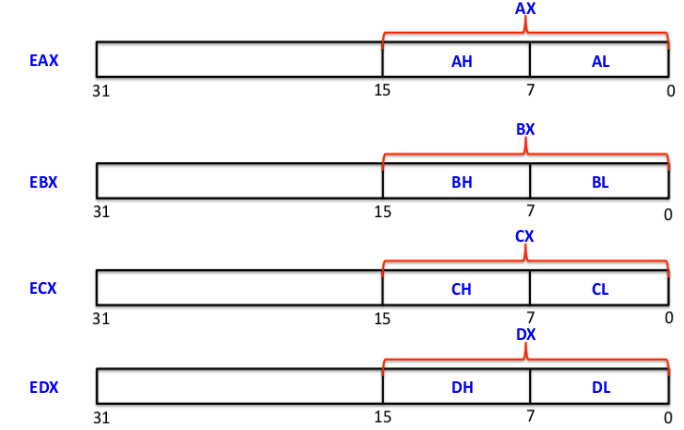
\includegraphics[width=300px]{registers.png}
\end{frame}

\begin{frame}{EFLAGS/RFLAGS}
\begin{itemize}
    \item Специальный регистр, каждый бит которого — какой-то флаг
    \item Нельзя записать значение напрямую, только косвенно через команды
    \item Два вида флагов: системные и арифметические
    \item Первые отвечают за текущие настройки поведение процессора
    \item Вторые предназначены для conditional jumps
\end{itemize}
\end{frame}

\begin{frame}{Если очень хочется перезаписать EFLAGS/RFLAGS}
\begin{itemize}
    \item \asm{pushf} кладёт EFLAGS на стек
    \item \asm{popf} восстанавливает EFLAGS со стека
\end{itemize}
\end{frame}

\begin{frame}{EFLAGS/RFLAGS}

\includegraphics[width=300px]{eflags.png}
\end{frame}

\begin{frame}{x86 memory segmentation}
\begin{itemize}
    \item Изначально x86 — 16-битная архитектура => только 64 Kb памяти адресуется
    \item Сегментные регистры: CS, DS, SS, ES, FS, GS.
    \item $addr = segment * 16 + offset$
    \item \asm{mov es:cx, 15h}
    \item FS и GS до сих пор используются :)
\end{itemize}
\end{frame}

\begin{frame}{Stack}
\begin{itemize}
    \item Реализуется через память
    \item Стек растёт обратно адресам (самый первый элемент в стеке имеет самый большой адрес)
    \item RSP указывает на последний занятый байт
    \item \asm{push} = \asm{sub rsp, size}; \asm{mov [rsp], op}
    \item \asm{pop} = \asm{mov op, [rsp]}; \asm{add rsp, size}
\end{itemize}
\end{frame}

\begin{frame}{Stack frame}
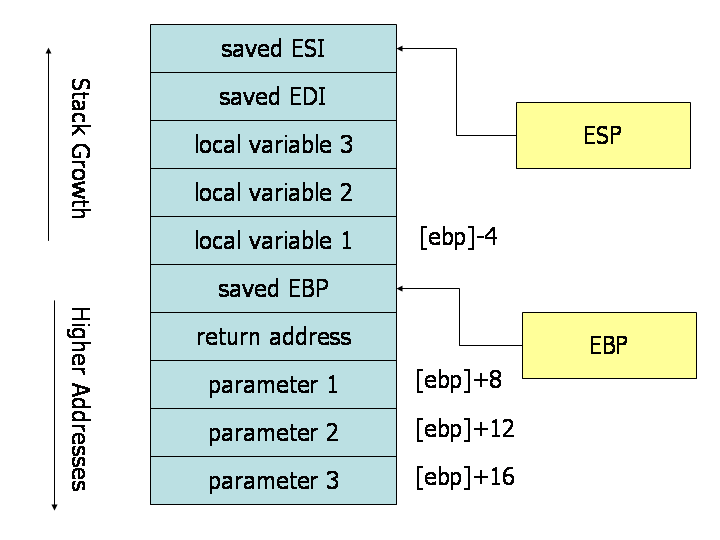
\includegraphics[width=300px]{stack.png}
\end{frame}

\begin{frame}{Calling conventions}
\begin{itemize}
    \item Соглашения о том, как реализуются вызовы функций
    \item Определяют где лежат аргументы и кто их сохраняет, выравнивание стека итд
    \item Под разными платформами и ОС — разные
    \item System V ABI (application binary interface)
    \item Можете придумать свои, но тогда придётся переписать компиляторы :)
\end{itemize}
\end{frame}


\qrlinkframe{Про инструкции}{https://www.felixcloutier.com/x86/}
\qrlinkframe{Intel manual}{https://software.intel.com/content/www/us/en/develop/articles/intel-sdm.html}

\begin{frame}{Как загружается компьютер?}
\begin{itemize}
    \item POST = Power-On Self Test
    \item BIOS ищет девайсы (партиции диска), помеченные boot-флагом и ищет там специальную MBR-запись в нулевом секторе диска
    \item 512-байтный сектор загружается по специальному адресу в память
    \item Процессор прыгает на этот адрес и начинается выполнение вашей ОС
    \item Интересный факт: так как питание процессора может быть не отключено (нажали на reset), то значения регистров могут быть от старого запуска
\end{itemize}
\end{frame}

\begin{frame}{Загрузчики}
\begin{itemize}
    \item Иногда бывает dual boot: Windows + Linux
    \item Не хочется, чтобы ОС реализовывала всю эту загрузку сама
    \item Загрузчик (например, GRUB) ставится на диск, а ОС загружается уже из файла на диске
    \item Загрузчик умеет работать с некоторыми файловыми системами и форматами ядер (ELF + бинарный формат)
\end{itemize}
\end{frame}

\begin{frame}{Real, protected и long mode}
\begin{itemize}
    \item Это различные режимы x86 процессоров, каждый обратно совместим с предыдущим
    \item После загрузки MBR вы находитесь в real mode — самый древний 16-битный режим
    \item Затем ОС делает подготовительные шаги и переходит в protected mode
    \item Аналогично с long mode
    \item Сделано это для того, чтобы на современных процессорах можно было запускать старые ОС (обратная совместимость)
\end{itemize}
\end{frame}

\begin{frame}{Real mode}
\begin{itemize}
    \item Отсутствует виртуальная память => нет прав на память, она вся RWX
    \item Сегментная адресация => максимум 1 Мб памяти адресуем
    \item Можно использовать специальные BIOS functions для доступа к периферии
\end{itemize}
\end{frame}

\begin{frame}{Protected mode}
\begin{itemize}
    \item Использует 32ух битные адреса
    \item Виртуальная память и страничная адресация
    \item Поддерживает механизм привилегий (т.н. кольца, rings)
    \item Поддержка кооперативной многозадачности из коробки (TSS = task state segment)
\end{itemize}
\end{frame}

\begin{frame}{Виртуальная память и страничная адресация}
\begin{itemize}
    \item Вся физическая память разделена на \emph{фреймы} — куски размером 4096 байт
    \item Вся виртуальная память аналогично разделена на \emph{страницы}
    \item Трансляцией виртуальной памяти в физическую занимается \emph{memory management unit} (MMU)
\end{itemize}
\end{frame}

\begin{frame}{Page tables}
\begin{itemize}
    \item Специальные структуры, которые хранят отображение виртуальной памяти в физическую
    \item Всего существует $2^{52}$ страниц памяти
    \item Если каждая страница описывается 8 байтами, то такая структура занимает $2^{60}$ байт в памяти
    \item Нужен более экономный способ хранить это отображение
\end{itemize}
\end{frame}

\begin{frame}{Multi-level page tables}
\begin{itemize}
    \item Идея: давайте сделаем таблицы многоуровневыми — сначала поделим всё пространство на части, каждую из этих частей ещё на части итд
    \item Не храня лишние «дыры» мы будем экономить место
    \onslide<2-> \item Под x86-64 используются четырёхуровневые таблицы: P4, P3, P2, P1.
    \onslide<2-> \item Каждая таблица занимает ровно 4096 байт и содержит 512 записей (\emph{PTE = page table entry}) по 8 байт
    \onslide<2-> \item Каждая запись ссылается на индекс в следующей таблице, последняя таблица ссылается на адрес фрейма
\end{itemize}
\end{frame}

\begin{frame}{Что хранится в PTE?}
\begin{itemize}
    \item Индексация следующей таблицы или фрейма не занимает все 8 байт PTE
    \item Кроме неё в PTE есть ещё специальные \emph{флаги страниц}
    \item Например, 1-ый бит отвечает за то, будет ли страница доступна на запись
    \item 63ий -- за то, будет ли процессор исполнять код на этой странице
    \item Также в некоторые биты процессор сам пишет флаги, например, dirty-бит устанавливается всегда, когда происходит запись в страницу
    \item Флаги имеют иерархическую видимость: если в P2 writeable-бит равен 0, а в P4 -- 1, то страница будет доступна на запись
\end{itemize}
\end{frame}

\begin{frame}{Устройство виртуального адреса}
\begin{itemize}
    \item На текущий момент x86-64 позволяет адресовать 48 бит физической памяти
    \item Старшие биты (с 48 по 63) должны быть sign extended копии 47ого бита
    \item Следующие биты (с 38 по 47) адресуют PTE в P4
    \item Биты с 29 по 37 адресуют PTE в P3
    \item Биты с 21 по 28 адресуют PTE в P2
    \item Биты с 12 по 20 адресуют PTE в P1, которая ссылает непосредственно на фрейм
    \item Биты с 0 по 11 адресуют смещение внутри фрейма
\end{itemize}
\end{frame}

\begin{frame}{Устройство виртуального адреса}
\center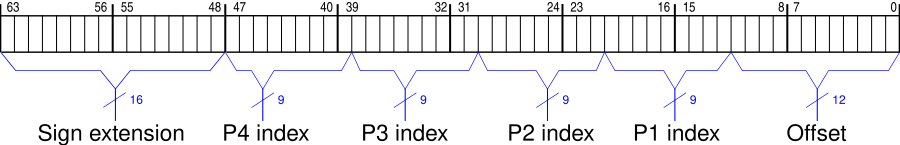
\includegraphics[width=325px]{x86_address_structure.png}
\end{frame}

\begin{frame}{Устройство виртуального адреса}
\center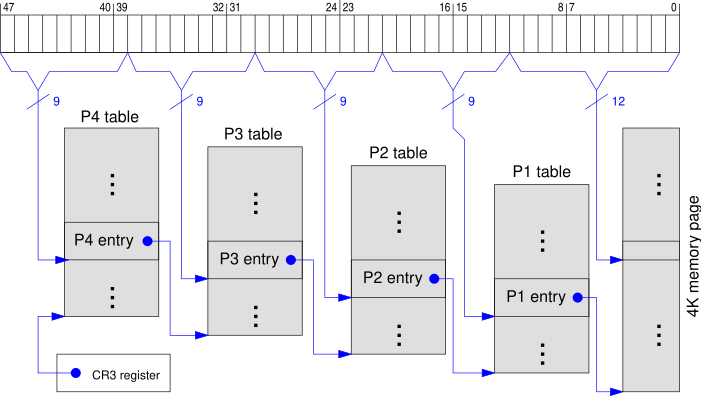
\includegraphics[width=325px]{X86_Paging_64bit.png}
\end{frame}

\begin{frame}{ОС и таблицы страниц}
\begin{itemize}
    \item Операционная система хранит таблицы страниц для каждого процесса
    \item Таблица страниц переключается каждый раз при context switch
    \item Физический адрес текущей P4 хранит специальный регистр CR3 (такие регистры называются \emph{MSR = model specific registers})
    \item В реальности каждое обращение к памяти не вызывает прыжки по таблицам, оно кэшируется в \emph{TLB = translation lookaside buffer}
    \item При context switch TLB полностью сбрасывается
\end{itemize}
\end{frame}

\begin{frame}{Выделение памяти: on-demand paging}
\begin{itemize}
    \item Современные ОС не выделяют всю запрошенную память сразу
    \item Вместо этого используется on-demand paging
    \item Если страницы нет в текущем memory mapping'е, то процессор сгенерирует специальное исключение, называемое \emph{page fault}'ом
    \item Идея состоит в том, чтобы детектировать с помощью page fault'ов реальные обращения к памяти и только тогда её выделять
\end{itemize}
\end{frame}

\begin{frame}{Прерывания процессора}
\begin{itemize}
    \item Могут выполниться после любой инструкции процессора
    \item Специальные участки кода с наибольшим приоритетом
    \item Прерывание в прерывании, ух!
    \item Вызываются ошибками памяти (обращение к несуществующей странице, запись в readonly страницу)
    \item Или событиями от периферийных устройств (сетевая карта, клавиатура)
    \item Одно из самых важных для ОС прерываний — timer interrupt
\end{itemize}
\end{frame}


\begin{frame}
\center\Huge{Спасибо!}
\end{frame}


\end{document}
